\documentclass[11pt,a4paper]{article}
\usepackage[spanish,es-nodecimaldot]{babel}	% Utilizar español
\usepackage[utf8]{inputenc}					% Caracteres UTF-8
\usepackage{graphicx}						% Imagenes
\usepackage[hidelinks]{hyperref}			% Poner enlaces sin marcarlos en rojo
\usepackage{fancyhdr}						% Modificar encabezados y pies de pagina
\usepackage{float}							% Insertar figuras
\usepackage[textwidth=390pt]{geometry}		% Anchura de la pagina
\usepackage[nottoc]{tocbibind}				% Referencias (no incluir num pagina indice en Indice)
\usepackage{enumitem}						% Permitir enumerate con distintos simbolos
\usepackage[T1]{fontenc}					% Usar textsc en sections
\usepackage{amsmath}						% Símbolos matemáticos
\usepackage{menukeys}

\newcommand{\shellcmd}[1]{\indent\indent\texttt{\footnotesize\$ #1}\\}

% Comando para poner el nombre de la asignatura
\newcommand{\asignatura}{Sistemas Gráficos}
\newcommand{\autor}{Vladislav Nikolov Vasilev}
\newcommand{\titulo}{Pac-Man 3D}
\newcommand{\subtitulo}{Manual de usuario}
\newcommand{\rama}{Ingeniería del Software}

% Configuracion de encabezados y pies de pagina
\pagestyle{fancy}
\lhead{\autor{}}
\rhead{\asignatura{}}
\lfoot{Grado en Ingeniería Informática}
\cfoot{}
\rfoot{\thepage}
\renewcommand{\headrulewidth}{0.4pt}		% Linea cabeza de pagina
\renewcommand{\footrulewidth}{0.4pt}		% Linea pie de pagina

\begin{document}
\pagenumbering{gobble}

% Pagina de titulo
\begin{titlepage}

\begin{minipage}{\textwidth}

\centering

%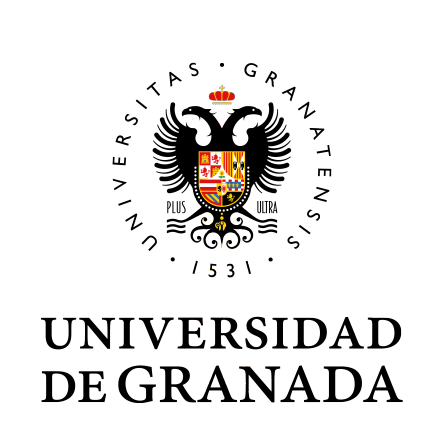
\includegraphics[scale=0.5]{img/ugr.png}\\

\includegraphics[scale=0.3]{img/logo_ugr.jpg}\\[1cm]

\textsc{\Large \asignatura{}\\[0.2cm]}
\textsc{GRADO EN INGENIERÍA INFORMÁTICA}\\[1cm]

\noindent\rule[-1ex]{\textwidth}{1pt}\\[1.5ex]
\textsc{{\Huge \titulo\\[0.5ex]}}
\textsc{{\Large \subtitulo\\}}
\noindent\rule[-1ex]{\textwidth}{2pt}\\[3.5ex]

\end{minipage}

%\vspace{0.5cm}
\vspace{0.7cm}

\begin{minipage}{\textwidth}

\centering

\textbf{Autor}\\ {\autor{}}\\[2.5ex]
\textbf{Rama}\\ {\rama}\\[2.5ex]
\vspace{0.3cm}


\includegraphics[scale=0.3]{img/etsiit.jpeg}

\vspace{0.7cm}
\textsc{Escuela Técnica Superior de Ingenierías Informática y de Telecomunicación}\\
\vspace{1cm}
\textsc{Curso 2019-2020}
\end{minipage}
\end{titlepage}

\pagenumbering{arabic}
\tableofcontents
\thispagestyle{empty}				% No usar estilo en la pagina de indice

\newpage

\setlength{\parskip}{1em}

\section{¿Qué es \texttt{Pac-Man 3D}?}

\texttt{Pac-Man 3D} es la versión 3D del clásico juego de recreativas \texttt{Pac-Man}, el cuál
apareció por primera vez a principios de la década de los 80. Esta nueva versión está implementada
en \texttt{JavaScript}, de forma que se puede jugar en cualquier navegador web.

\section{¿En qué consiste el juego?}

En el juego se toma el control de \texttt{Pac-Man}, un personaje amarillo que abre y cierra
su boca al moverse. Existen también otros elementos dentro del juego, como los puntos pequeños y
los grandes, los cuáles tienen un color amarillo pálido; los muros, los cuáles son de color azul
oscuro; y cuatro fantasmas, los cuáles son los enemigos del juego y tienen diferentes colores.

En la siguiente figura puede observarse un ejemplo de partida, con todos los elementos que se
pueden ver en pantalla:

\begin{figure}[H]
	\centering
	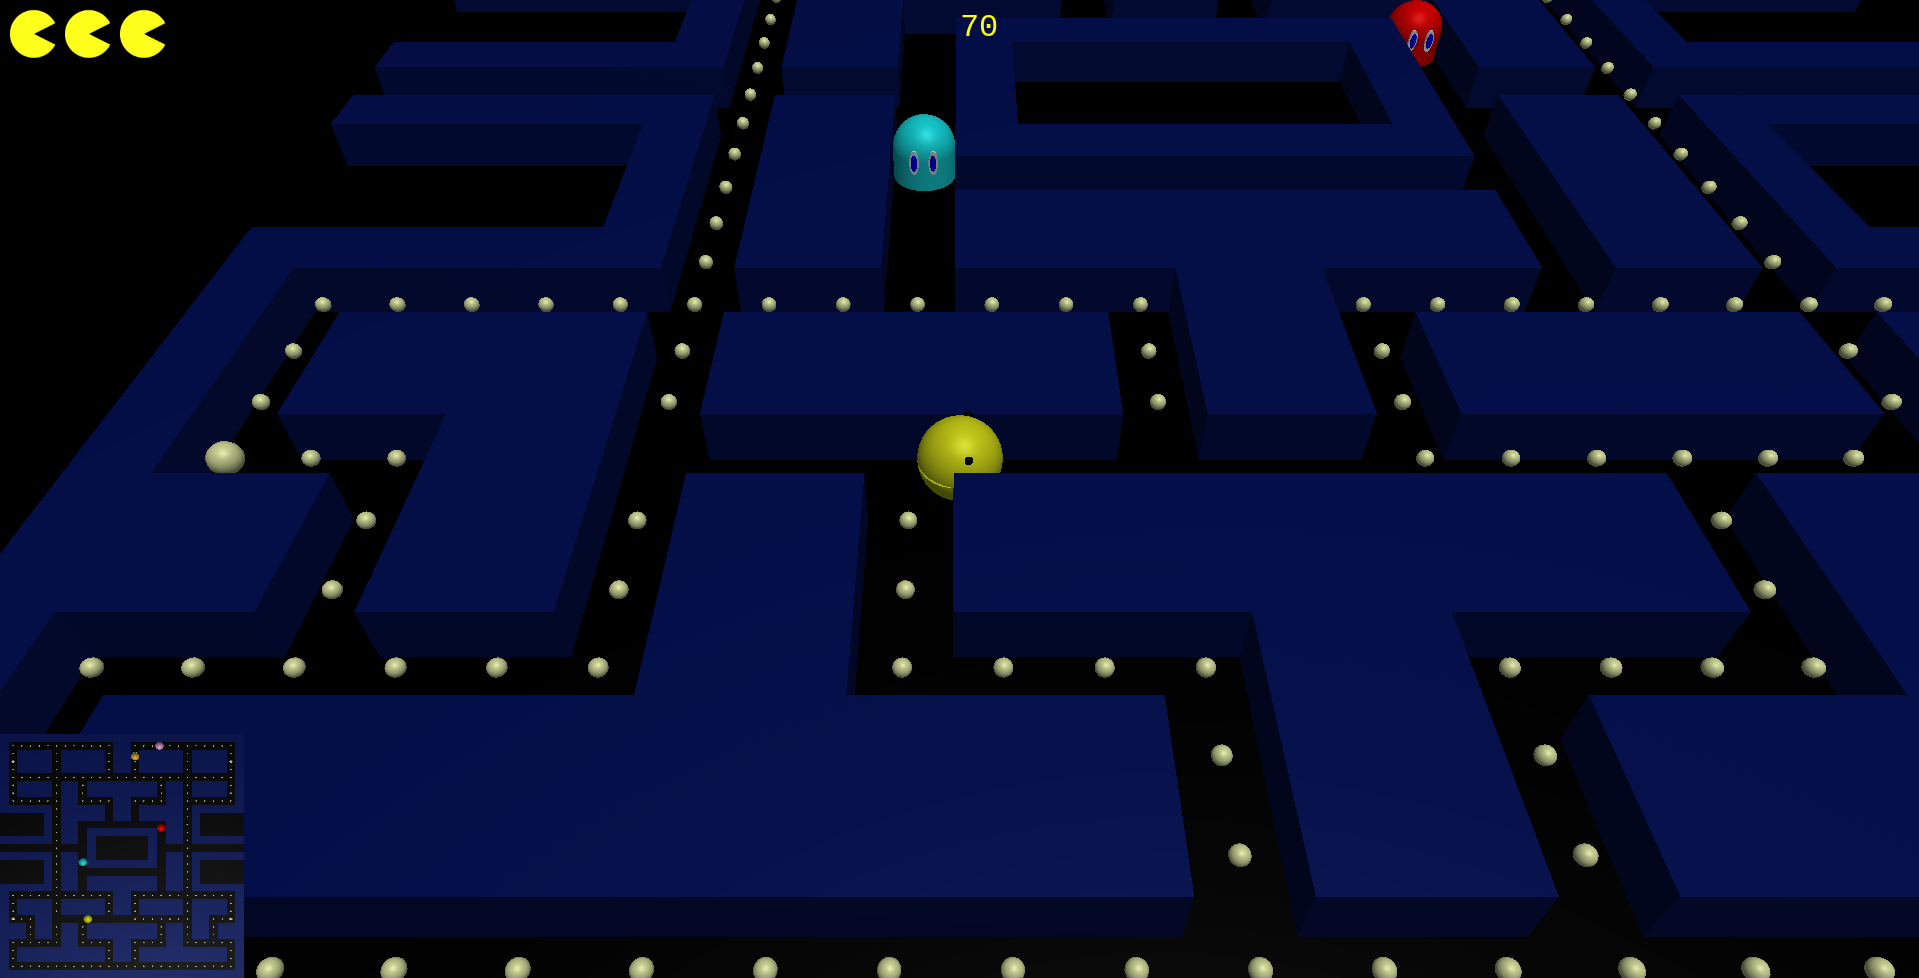
\includegraphics[scale=0.3]{img/pac-man-game}
	\caption{Ejemplo de una partida del juego.}
	\label{fig:pac-man}
\end{figure}

En la esquina superior izquierda pueden apreciarse tres iconos de \texttt{Pac-Man}, los cuáles
representan las vidas restantes del personaje. El personaje tiene tres vidas al comienzo de
la partida, y cuando las pierde todas, se acaba la partida. Se pierde una vida cuando el
personaje colisiona con alguno de los fantasmas. Cuando el personaje muere, reaparece en la
posición inicial, y tras 2 segundos, empieza a moverse de nuevo.

En la esquina inferior derecha se puede apreciar un minimapa, el cuál muestra una vista aérea en
tiempo real de todo el escenario, de forma que se pueda comprobar fácilmente dónde está cada
elemento del juego.

Por último, arriba en el centro está la puntuación. Cada vez que el personaje se come un punto
la puntuación se ve incrementada en una determinada cantidad.
Comerse un \textbf{punto pequeño} le aporta \textbf{10 puntos},
mientra que comerse un \textbf{punto grande} le da \textbf{50 puntos}. Adicionalmente, al comerse
un punto grande, el personaje obtiene la capacidad de comerse a los fantasmas durante 8 segundos.
Comerse a los fantasmas durante este período proporciona una serie de puntos: 200 puntos el
primero, 400 el segundo, 800 el tercero y 1600 el cuarto. Cuando el personaje se come a un
fantasma éste reaparecerá al momento en la posición correspondiente, y no podrá volver a
comérselo hasta que no se coma otro punto grande. Si el jugador se come otro punto grande antes
de que el efecto del anterior haya expirado se reiniciará el efecto: todos los fantasmas, tanto
los que ya se ha comido como los que no volverán a ser comestibles durante el mismo período de
tiempo y se reiniciará la cantidad de puntos que ofrece cada fantasma al comérselo, comenzando
por tanto de nuevo en 200.

Una vez que el personaje se haya comido todos los puntos se reinicia el nivel, conservando
la puntuación obtenida y las vidas restantes, recolocando todos los puntos que había anteriormente
en el escenario, reseteando la posición del personaje a la inicial e incrementando ligeramente
la velocidad a la que se mueven tanto el personaje como los fantasmas, siempre y cuando dichas
velocidades no hayan excedido un determinado límite. Por tanto, el \textbf{objetivo} es, con las
vidas disponibles, \textbf{conseguir la máxima puntuación posible}.

Como información adicional con respecto al juego, se pueden destacar tres cosas:

\begin{enumerate}
	\item El personaje es ligeramente más rápido que los fantasmas, de manera que pueda
	escapar de éstos si es perseguido.
	\item El comportamiento de los fantasmas es aleatorio. Esto hace que la dificultad del
	juego no sea muy elevada. No es como en el juego original, donde cada fantasma tiene un
	comportamiento diferente.
	\item En la fila central del mapa, el extremo izquierdo está conectado con el derecho y
	viceversa. Esto ofrece una ruta rápida tanto para los fantasmas como para el personaje para
	ir de la parte derecha del mapa a la izquierda en poco tiempo.
\end{enumerate}

\section{¿Cómo se puede jugar?}

Se puede jugar de dos maneras distintas:

\begin{itemize}[label=\textbullet]
	\item Por una parte, si se tiene el código del proyecto, basta con situarse en el directorio
	donde se encuentre el archivo \texttt{index.html}. Una vez ahí, se abre una terminal en dicho
	directorio y se ejecuta el siguiente comando:
	
	\shellcmd{python -m SimpleHTTPServer}
	
	Esto creará un nuevo servidor local en el puerto 8000. Para acceder a él, basta con
	entrar a cualquier navegar y acceder a la siguiente URL: \texttt{localhost:8000}. De
	esta forma, se empezará una nueva partida, la cuál se está ejecutando en local.
	\item Otra opción, en caso de no querer ejecutar un servidor en local y acceder a él, consiste
	en acceder a la siguiente página web, donde el juego se encuentra desplegado:
	\url{https://vol0kin.github.io/PacMan3D}.	
\end{itemize}

\section{¿Cómo se interactúa con el juego?}

La interacción con el juego se realiza mediante el teclado. Pulsando unas determinadas teclas
se cambia la orientación del personaje, de forma que se mueve o se intenta mover en la dirección
deseada, dependiendo de si choca contra un muro o no. Dichas teclas son las siguientes:

\begin{itemize}
	\item La tecla \keys{W} permite orientar al personaje hacia \textbf{arriba}.
	\item La tecla \keys{A} permite orientar al personaje hacia la \textbf{izquierda}.
	\item La tecla \keys{S} permite orientar al personaje hacia \textbf{abajo}.
	\item La tecla \keys{D} permite orientar al personaje hacia la \textbf{derecha}.
\end{itemize}

Basta con realizar una pulsación de la tecla para cambiar la orientación del personaje a la
deseada. El movimiento del personaje es automático en función de la orientación. El cambio
de orientación se puede hacer en cualquier momento, independientemente de si en la nueva
dirección de movimiento hay un muro o no.
Es importante destacar que el cambio de dirección puede efectuarse una vez que el personaje
haya comenzado a moverse. Esto significa que durante el tiempo en el que se inicia la partida y
suena la música de inicio y durante dos segundos después de reaparecer no puede cambiarse la
orientación del personaje.

\end{document}

